\todo{make introduction to the chapter}
\section{Introduction}
Android is mobile operating system developed by Google. It's opensource system based on the Linux kernel mainly used in mobile devices such as smartphones, tablets and smart watches, but it can be found also in devices such as set-top boxes, media players and other electronics.

Android, Inc. was founded in California USA in 2003. Google, Inc. bought Android two years later. In 2007, Google acquired several patents in the field of mobile devices. The same year on November 5, there is official presentation of an association of companies formed the Open Handset Alliance which aims to create open standards in mobile devices. The first smartphone running Android released on October 22, 2008.

Table \ref{androidHistory} presents a brief history of an operating system Android. There are described release dates of major versions, the numbering which change by the size of the system modifications, code names represented by a popular foods from version 1.5 and API levels in the last column.

\begin {table}[h!]
    \begin{tabular}{|l|c|l|c|}
    \hline
    {\bf Release date}  & {\bf Version} & {\bf Codename}        & {\bf API level}   \\
    \hline \hline
    September 23, 2008  & 1.0 -- 1.1    & ---                   & 1 -- 2            \\
    \hline
    April 27, 2009      & 1.5           & Cupcake               & 3                 \\
    \hline
    September 15, 2009  & 1.6           & Donut                 & 4                 \\
    \hline
    October 26, 2009    & 2.0 -- 2.1    & Eclair                & 5 -- 7            \\
    \hline
    May 20, 2010        & 2.2 -- 2.2.3  & Froyo                 & 8                 \\
    \hline
    December 6, 2010    & 2.3 -- 2.3.7  & Gingerbread           & 9 -- 10           \\
    \hline
    February 22, 2011   & 3.0 -- 3.2    & Honeycomb             & 11 -- 13          \\
    \hline
    October 18, 2011    & 4.0 -- 4.0.4  & Ice Cream Sandwich    & 14 -- 15          \\
    \hline
    July 9, 2012        & 4.1 -- 4.3    & Jelly Bean            & 16 -- 18          \\
    \hline
    October 31, 2013    & 4.4 -- 4.4.4  & KitKat                & 19 -- 20          \\
    \hline
    November 12, 2014   & 5.0 -- 5.0.2  & Lollipop              & 21                \\
    \hline
    \end{tabular}
    \centering
    \caption{Android version history}
    \label{androidHistory}
\end{table}

\section{Architecture}
The following section describes the architecture of Android system which consists from six layers. Figure~\ref{androidArchitecture} shows this architecture starting with kernel layer and ending with user application.
\\
\begin{figure}[h!]
    \centering
    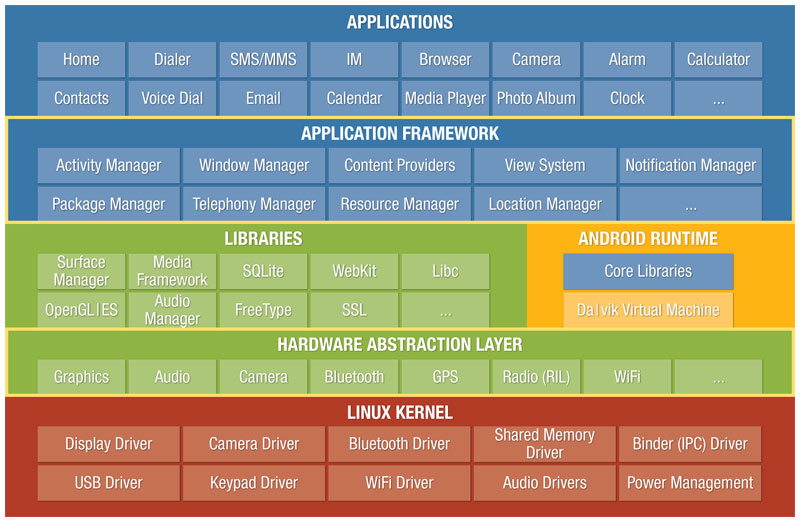
\includegraphics[scale=0.55]{fig/android_architecture.jpg}
    \caption{Android architecture \cite{AndroidArch}}
    \label{androidArchitecture}
\end{figure}

\paragraph{Linux kernel}
The lowest layer stands between hardware devices and other architectural layers. Android is based on special version of Linux kernel and several accessories such as memory management system, the Binder IPC driver and others. Since the beginning, Android was built on the Linux 2.6 kernel but the latest Android version runs on the kernel 3.4.

\paragraph{Hardware abstraction layer}
Hardware abstraction layer (HAL) is standart interface which allows Android system calls to drivers layer while he does not care what is the implementation of drivers and hardware in the lower layers. For each piece of hardware should be a driver and matching HAL providing hardware options.

\paragraph{Libraries}
Above the HAL is a layer of native libraries. These libraries are written in C or C ++ and can be accessed through the Android Standard Development Kit (SDK), but if direct access is required, it is possible to do that through the Native Development Kit (NDK). The HAL includes the following libraries:

\begin{itemize}
\item \textbf{Surface manager} -- library for composing different drawing surfaces windows on the screen
\item \textbf{Media Framework} -- provides various multimedia codecs for playing and recording video in many formats
\item \textbf{SQLite} -- a database engine for the use in data storage
\item \textbf{WebKit} -- a browser engine for displaying web content
\item \textbf{Libc} -- the standard library of the C programming language
\item \textbf{OpenGL ES} -- a library for support 2D and 3D graphics and hardware accelerated rendering
\item \textbf{Audio Manager} -- a library for working with sounds of device
\item \textbf{FreeType} -- a library for bitmap and vector font rendering
\item \textbf{SSL} -- a library for the use of encryption protocol for secure Internet communications
\end{itemize}

\paragraph{Android runtime}
Android runtime layer is located next to native libraries. This layer consist of two parts. The first one is the Core Libraries and the second one is the Dalvik Virtual Machine. The Core libraries can be further subdivided into two parts: Java Libraries and Android libraries.

\paragraph{Application framework}
Application framework layer provides many high-level services to applications in the form of Java libraries. For developers, this is the most important layer that allows access to the device services. The Application framework includes the following parts:
 
\begin{itemize}
\item \textbf{Activity manager} -- controls all aspects of running activities. It manages all Services and Activities  described in Section~\ref{AppStructure}.
\item \textbf{Windows manager} -- provides services for windows management such as visibility and arrangement. It also takes care about animation on the screen.
\item \textbf{Content Providers} -- allows to work with the contents of other applications, they encapsulate the data, and provide mechanisms for defining data security.
\item \textbf{View System} -- a set of basic blocks that is used to build the application user interface. The basis of every graphical component is View class which is represented by a rectangular area on the screen.
\item \textbf{Notification manager} -- provides the possibility how to inform the user about some action that happened in the background. Notifications can take different forms like LED flashing, vibrating, ringing or notification on display.
\item \textbf{Package manager} -- allows obtaining of various information about applications that are currently installed on device.
\item \textbf{Telephony manager} -- provides access to telephone services of device. These services include SIM card, network, cellphone and other information.
\item \textbf{Resource manager} -- allows access to non-code resources such as color settings, layouts and strings. Separating of resources from code helps to better management of various characteristic withour modifying code.
\item \textbf{Location manager} -- provides access to the location services. These services allow periodical receiving of geographic coordinates and therefore it is possible to track device current location.
\end{itemize}

\paragraph{Applications}
The last and highest layer consists of the application itself. These comprise both pre-installed applications and applications that have been added over time from the Android store or an other way.

\section{Android runtime}
Both Android runtime and JRE include a virtual machine and Java SE API. In case of Android runtime, Android contains special virtual machine named Dalvik Virtual Machine, API lacks several Java packages and classes and special Android libraries are included.

\subsubsection{Dalvik Virtual Machine (DVM)}
DVM is a virtual machine that is being developed since 2005 and it was included into the system due to the JVM was not licensed as open source at that time. The second reason was the optimization for mobile devices. 

Each application runs on Android devices within its own instance of DVM (i.e. not as a process in the Linux kernel).

Running applications on a virtual machine has many advantages. First, it operates in a sandbox and thus can not interfere with the operating system or to other applications. Secondly, it makes the application platform independent and therefore can be run on any hardware. Advantages include its DVM efficiency in memory usage and is thus better adapted for use on mobile devices.

The application code must be always transformed from a standard .java file into bytecode but it is different from Java applications from this point. Bytecode is not executed by DVM but instead bytecode is converted by dex tool to Dalvik executables (.dex format). The whole process is described in the Section~\ref{buildProcess}.


\paragraph{Java libraries}
Most of Android applications are written using Java. Android contains libraries based on Apache Harmony Project that is open source Java implementation. These libraries are a subset of the Java SE platform. They do not contain all of package. For example java.awt or java.swing libraries are replaced by Android user interface classes and packeges. More detailed comparison can be found in the Chapter~\ref{apis}.

\paragraph{Android libraries}
Android libraries are specific libraries that provide all the functionality of android devices. Libraries are written in Java and the following packages are included:

\begin{itemize}
\item android.app -- provides access to the application model and is the cornerstone of all applications
\item android.content -- classes for accessing and publishing data applications
\item android.database -- classes for data access and database manipulation 
\item android.graphics -- library for screen low-level 2D graphics drawing
\item android.hardware -- provide access to hardware features such as cameras and sensors
\item android.media -- library for handling with multimedia 
\item android.text -- library for manipulate and rendering of strings
\item android.util -- common tools such as data manipulation and time, conversions between numbers and strings, and more
\item android.view -- basic building library for building a graphical user interface
\item android.webkit -- libraries for working with web content
\end{itemize}

\section{Application structure}\label{AppStructure}
In this section we will describe the anatomy of the application, various components that are used for creating android applications.
%V této sekci budou popsány hlavní části aplikace. Budou popsány jednotivé komponenty které se používají oro tvorbu android aplikací.

\paragraph{Activities}%http://developer.android.com/guide/components/activities.html
Activities represent one single screen of user interface. Typically, after starting the application the main activity shows and from there we can run another activity or perform other operations. When you start a new activity, the previous one is stored in a LIFO stack. After pressing the back button is invoked again.
%Aktivity reprezentují jednu samotnou obrazovku živatelského rozhraní. Typicky po spuštění aplikace je zobrazena hlavní aktivita z které se pak mohou spouštět aktivity další, či provádět jiné operace. Když se spustí nová aktivita, ta předchozí je uschována v Last in first out zásobníku. Po stisknutí tlačítka zpět je znovu vyvolána.

\paragraph{Services}
Services are components that run in the background performing long-term tasks. They do not provide a user interface. Services may be still active in the background while running other applications. Example of services can be download content from the Internet while another application is running.
%Služby jsou komponenty, které beží na pozadí provádějící dlohotrvající operace. Neposkytují uživatelské rozhraní. Služby mohou být stále aktivní i na pozadí zatímco beží jiná aplikace. Příkladem služby může být stahování obsahu z internetu zatímco je spuštěná jiná aplikace.

\paragraph{Content providers} %http://developer.android.com/guide/components/fundamentals.html
Content providers store, load data and make it available for other applications. Through the content providers other applications may modify or manipulate specific data. An example might be a content provider that manages the contact information on the device.
%Content providers ukládají, načítají data a zpřístupňjí je pro všechny aplikace. Zkrz content providery mohou ostatní aplikace data modifikovat či s nimi manipulovat. Příkladem může být kontent provider který spravuje informace o kontaktech v zařízení.

\paragraph{Intents}
The application area is composed of activities and messages between them, which we call Intents. Intent consist of activities to be done and the parameter that is attached to it. We can divide intents into explicit and implicit. Explicit Intent contain action and intention to be made and platform will select the application. Implicit Intent also contain action and object but depends on which application the user chooses.
%Aplikační prostor je složen s aktivit a zpráv mezi nimi, které nazýváme intenty. Ty se skládájá z činnosti která se má vykonat a parametru který je k ní připojen. Intenty můžeme rozdělit na explicitní a implicitní. Explicitní intenty obsahují akci a záměr které se má provést a výběr aplikace už zařídí platforma.  Implicitní intenty obsahují také akci a objekt ale závisí na uživateli jakou aplikaci zvolí.

\paragraph{Broadcast receivers}
These are components which are used to listen notification from outside or from inside of the application. Reaction is formed by the type of notification: notification in the status bar, toast, or notification dialog box. An example might be a notification of incoming sms or low battery.
%Jsou to komponenty, které složí k nasloucháná oznámení z vnějšku popř. zevnitř aplikace. Podle typu oznámení následuje reakce: oznámeníve stavovém řádku, toast, či oznámení dialogovým oknem Příkladem může být oznámení o příchozí sms nebo nízkém stavu baterie.

\paragraph{Application Resources} %http://developer.android.com/guide/topics/resources/available-resources.html
Android application consists not only from source code but also from the resources that are separated from the code. These resources include:
%Android aplikace se skládá nejen ze drojových kódů ale také z resources, které jsou od kódu odděleny. Mezi tyto resourcy patří:
\begin{enumerate}
\item Animation Resources -- defines predefined animation
%definují předem stanovené animace
\item Color State List Resource -- defines color change based on the View state
%definují barvy měnící se na základě stávu View
\item Drawable Resources -- defines different graphics -- bitmaps or xml files
%definují různé grafiky s bitmapami nebo xml soubory
\item Layout Resource -- defines the layout of application components
%definují rozložení component aplikace
\item Menu Resource -- defines content of aplication menus
%definují obsah menu aplikace
\item String Resources -- defines string, string arrays
%definují řetězce, pole řetěztců.
\item Style Resource -- defines the appearance and format of ui elements.
%definují vzhled a formát ui elementů.
\item and other resources.
\end{enumerate}

\paragraph{Application Manifest} % http://developer.android.com/guide/topics/manifest/manifest-intro.html
Each application's root folder must have a file AndroidManifest.xml. This file contains information about the application with regard to Android. It should contain a unique package name for the application, the declaration of used components - activities, services. Then application permissions to the protected parts of the API (such as access to the camera, etc.). There also have to be declared a minimum level api, list of libraries with which the application is connected and other informations about application.
%Každá aplikace ve své rootovské složcě musí mít soubor AndroidManifest.xml. Tento soubor obsahuje informace o aplikaci s ohledem na systém Android. Měl by obsahovat unikátní jméno balíčku pro danou aplikacim deklaraci použitých komponent - aktivitm, služeb. Dále pak oprávnění aplikace ke chtáněným částem api (jako přístup k fotoaparátu apod). Také je potřeba deklarovat minimální úroveň api a seznam knihoven s kterými je aplikace propojena.

\section{Build System}\label{buildProcess}
Build System is the way how .apk package is produced from source code and resources. Apk file is the package file format used to distribute and install application software to Android. The entire process is automated by using Gradle scripts in the latest versions.
%Build System je způsob jakým se vyprodukuje ze zdrojového kódu a závislostí a reourců .apk balík. Celý tento proces je automatizován pomocí gradle skriptů ale je pro portování aplikací je dobré mu porozumět.

\subsection{Build Process}
Figure \ref{buildProcess} shows way of creating .apk package. The individual steps are these:
%Ná obrázku je možné vidět jakým způsobem probíhá vytváření .apk balíčku. Jednotlivé kroky jsou pak tyto:
\begin{enumerate}
\item The Android Asset Packaging Tool compile resource files and AndroidManifest.xml and produce R.java file, so it is possible to refer to the resources.
%The Android Asset Packaging Tool zkompiluje resource soubory jako jsou manifest a xml soubory a vyprodukuje R.java takže je možné se na resourcy odkazovat.
\item Aidl coverts all .aidl interfacese to java interfaces.
%Aidl konvertuje všechny .aidl rozhraní do java rozhraní
\item Whole code is compilated by java compilator. Outputs are .class files. 
%Všechen kód je zkompilován java kompilátorem, výstupem jsou .class soubory.
\item Dex tool converts .class and third-party files into Dalvik byte code.
%Nástroj dex převede .class soubory do Dalvik byte kodu. Stejně tak soubory třetích stran
\item All uncompiled resource (eg. Images), compiled resource and .dex files are sent to apkbuilderu which is pack them to .apk file.
%Všechny nokompilované resourcy (např. obrázky), kompilované resourcy a .dex soubory jsou poslany apkbuilderu aby je zabalil do .apk souboru.
\item Then .apk file must be signed.
%Poté musím byt .apk podepsán.
\item Finally, if the application is being signed in release mode, zipalign tool align the .apk file and thereby decreases memory usage
%Nakonec pokud je podepsán v release módu musí být zipalign nástrojem vyrovnán a tím se sníží paměťová náročnost.
\end{enumerate}

\begin{figure}[h!]
    \centering
    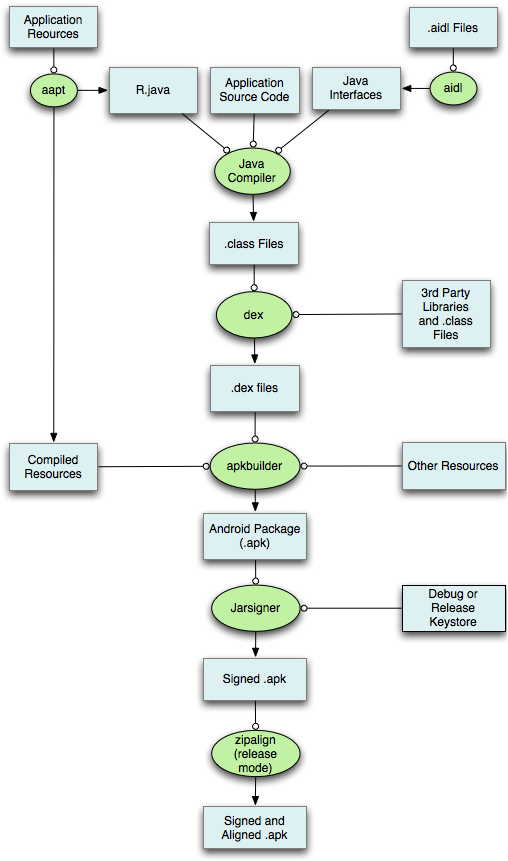
\includegraphics[scale=0.7]{fig/build.png}
    \caption{Build process}
\end{figure}



